\section{Efficiency calculations}
Measurements of the total selection efficiencies
$\eff{tot}(\btokpipimumu)$,
$\eff{tot}(\btopsitwosk)$,
$\eff{tot}(\btophikmumu)$, and
$\eff{tot}(\btojpsiphik)$,
must be made in order to determine the branching fractions for the decays \btokpipimumu and
\btophikmumu.
These efficiencies were calculated using simulated events; therefore, in order that the above
efficiencies are correct it is imperitive that the simulated events describe the data accurately.
Where there are discrepancies, the simulations must be corrected.

There are some variables which are known to be poorly described in simulation, particularly track
multiplicity and the \chisqvtx of the \Bp candidate.
The effects of these discrepancies are minimalised by reweighting simulated events using
the distributions of \btojpsikpipi.
Track multiplicity is known to be poorly described in simulation, generally the number of tracks is
less than in data, these discrepancies are illustrated in \Fig{fig:hhh:ntracks}.
Aside from the direct differencies, the low track multiplicity of in sumulated events is a
contributing factor of PID variables being badly described in simulations.

\begin{figure}
  \begin{center}
    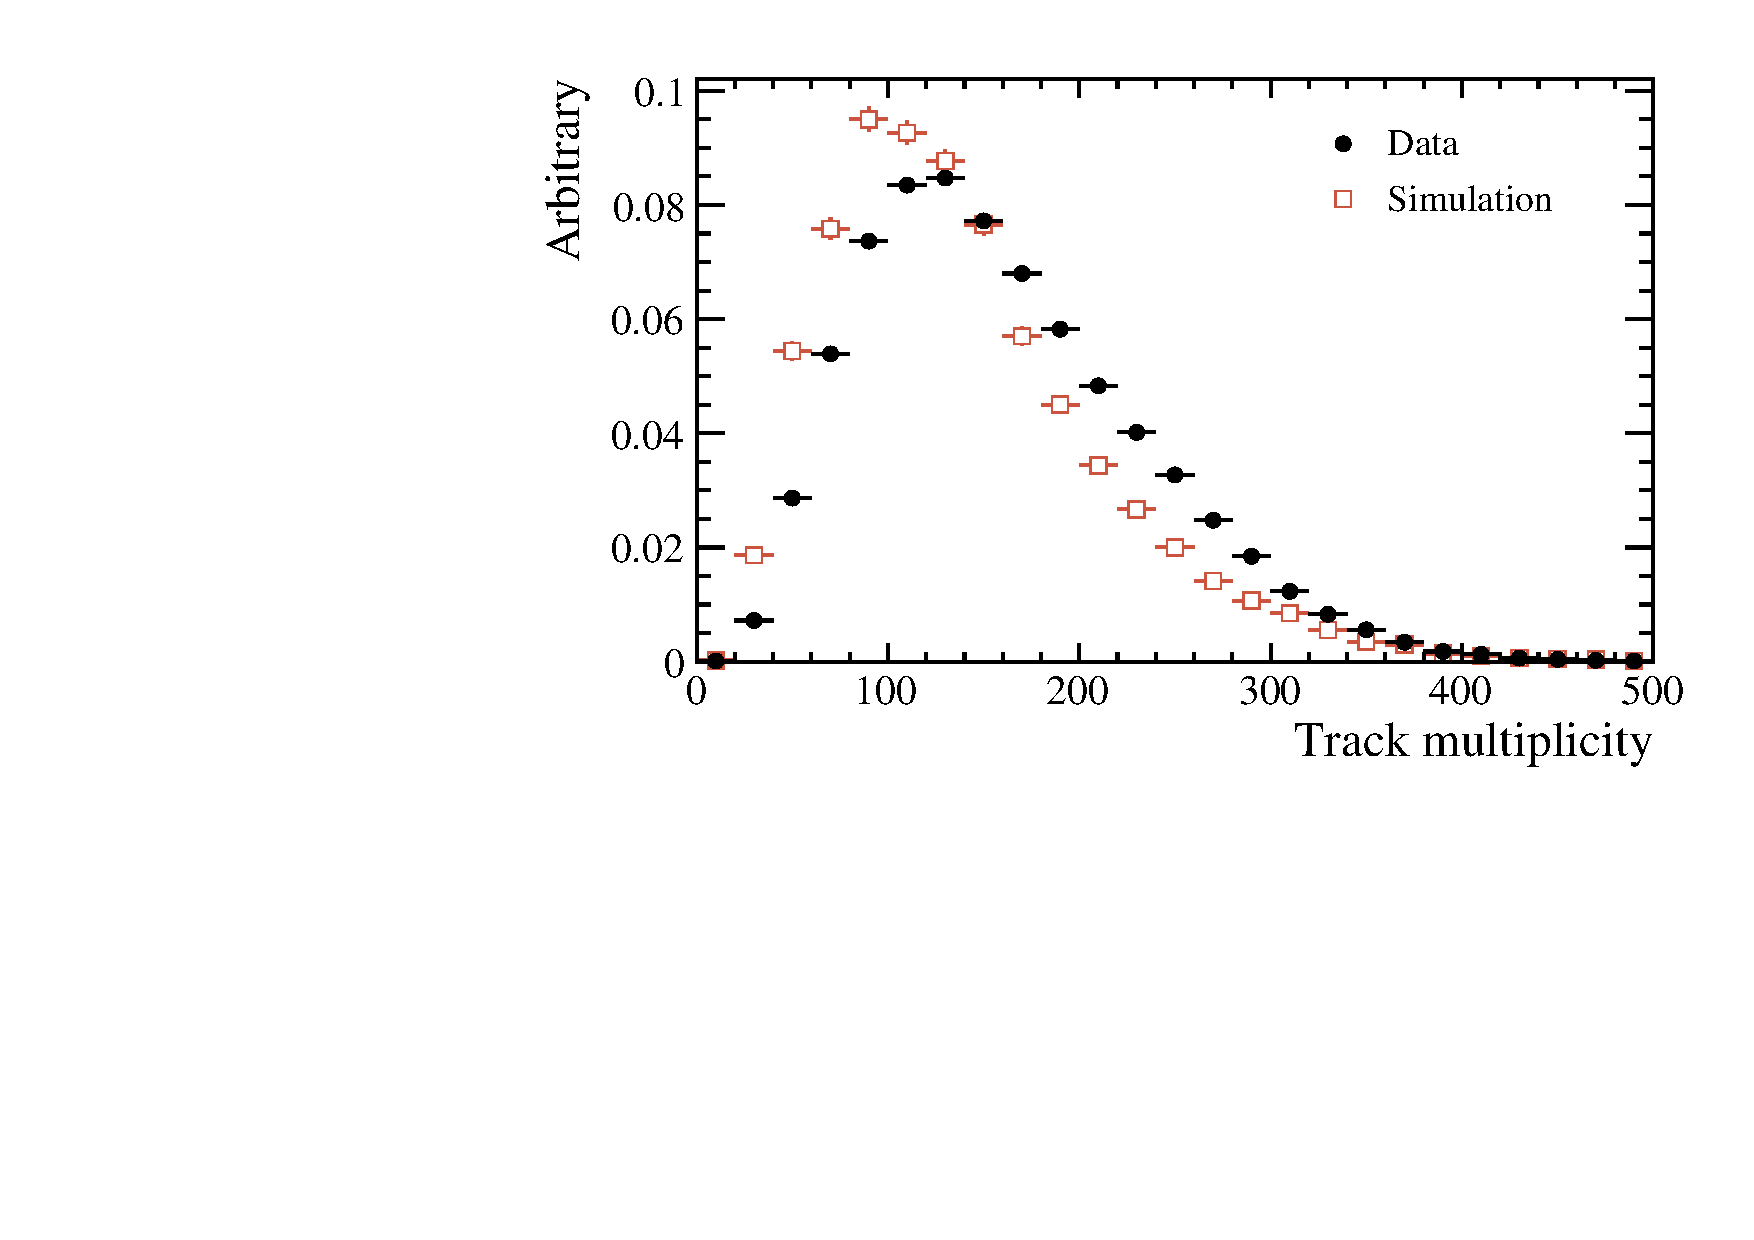
\includegraphics[width=0.48\textwidth]{ntracks}
    \caption{\small
      Distributions of track multiplicity for (black circles) data and (red squares) simulation.
      Simulated events are known to mis-model the track multiplicity, having a lower average number
      of tracks per event.
    }
    \label{fig:hhh:ntracks}
  \end{center}
\end{figure}

To ensure that efficiencies from PID cuts are determined accurately from simulation, the variables
must be corrected.
This is done with data driven methods, using highly pure samples of pions, kaons
and muons (which came from the decays \decay{\Dstarp}{\Dz\pip}, where \decay{\Dz}{\Km\pip}, and
\jpsitomumu).
For each track in the simulated \Bp candidate, a new PID variable is rasampled from PID
distributions of the pure track samples as a function of the track's $\eta$, $p$ and track
multiplicity.
Only required for kaons and pions, the muon PID distribution is well described in simulation.
Figure~\ref{fig:hhh:pid} shows the effect of this resampling technique, it is observed that the
simulated PID distributions that have been resampled matches data distributions much more than the
raw distributions; the differences that remain are accounted for in the systematic uncertainties.

\begin{figure}
  \begin{center}
    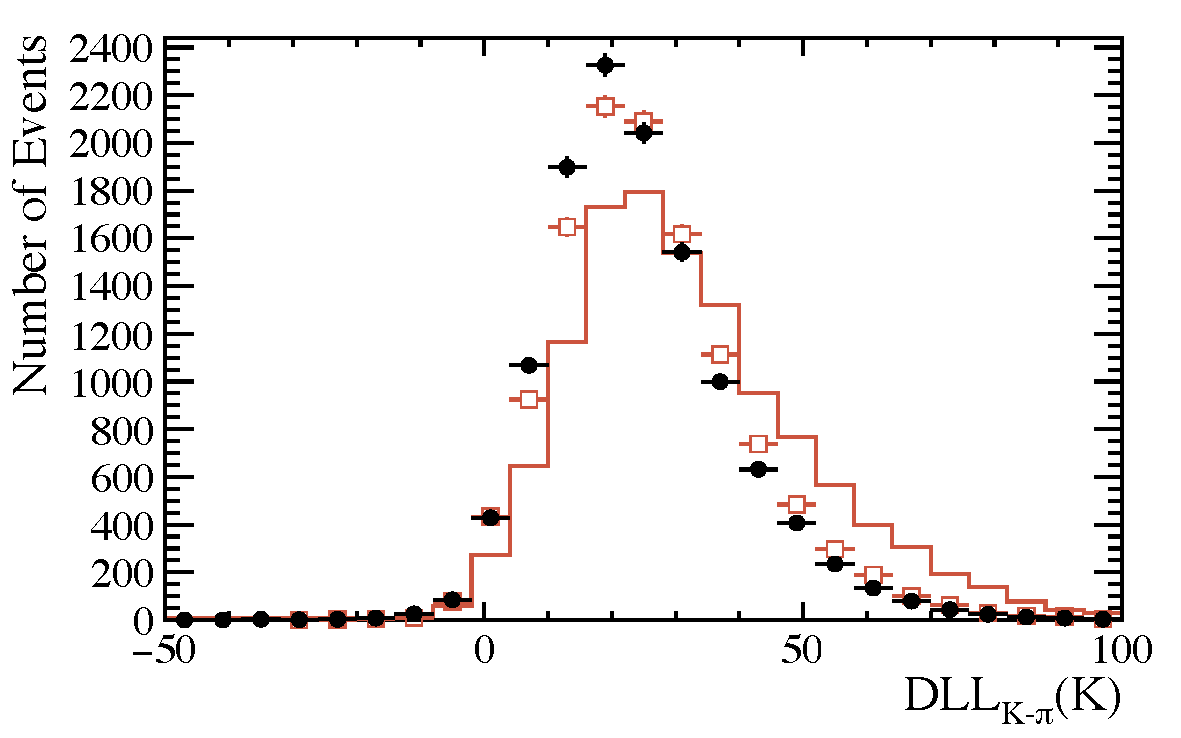
\includegraphics[width=0.48\textwidth]{pid_Kplus}
    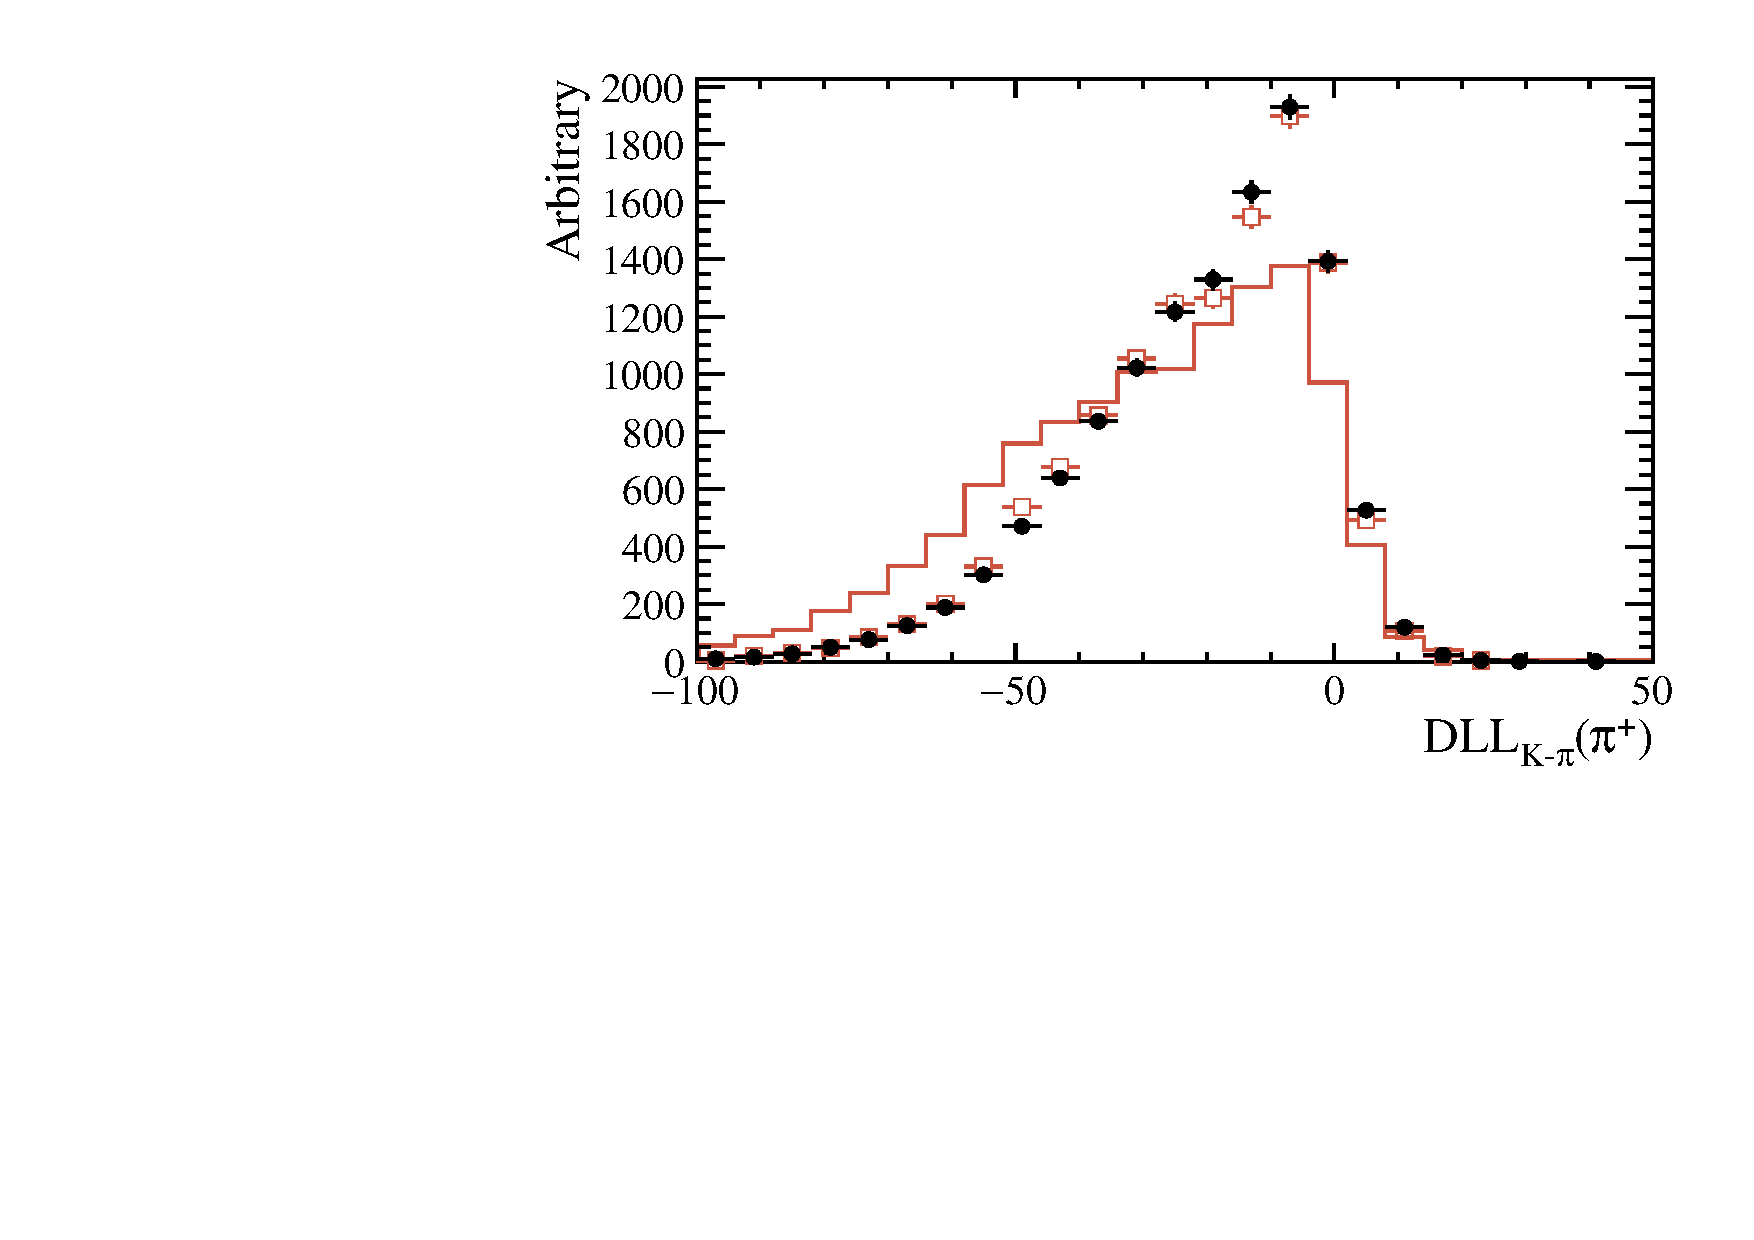
\includegraphics[width=0.48\textwidth]{pid_piplus}\\
    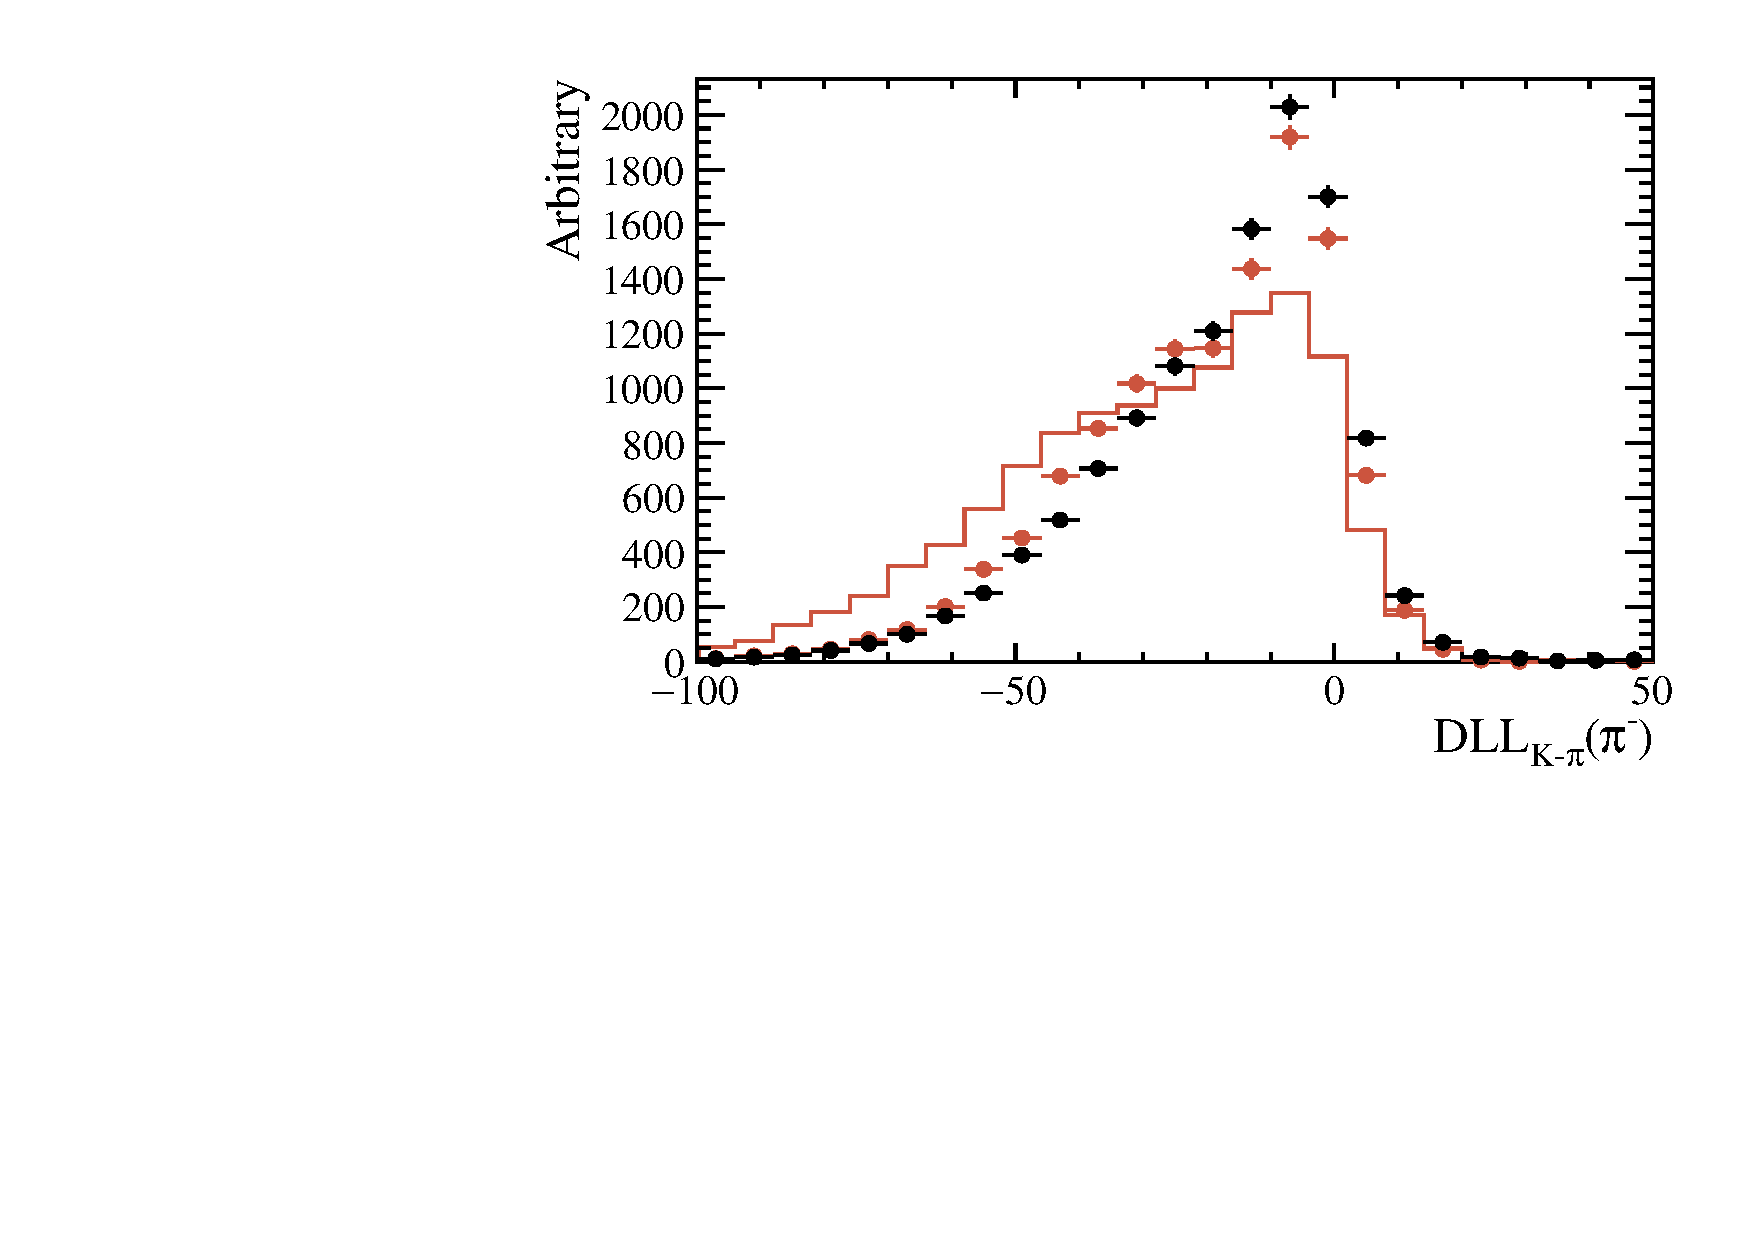
\includegraphics[width=0.48\textwidth]{pid_piminus}
    \caption{\small
      The effect of PID resampling for simulated tracks using pure samples of pions, kaons and
      muons.
      There is marked improvement in the similarity of the (black circles) \btojpsikpipi data and
      simulated events before (red line) resampling and after (red squares).
    }
    \label{fig:hhh:pid}
  \end{center}
\end{figure}

%Reweighting

Tracking efficiency varies depending upon the regions of the detector through which the paricle
passes...
These effects are different in data and simulation.



%Geometric efficiencies
%Tracking efficiencies and isMuon













After all the rewighting of simulated events, the BDT distributions are seen to be in agreement,
this is shown in \Fig{fig:kpipi:bdt}.

\begin{figure}
  \begin{center}
    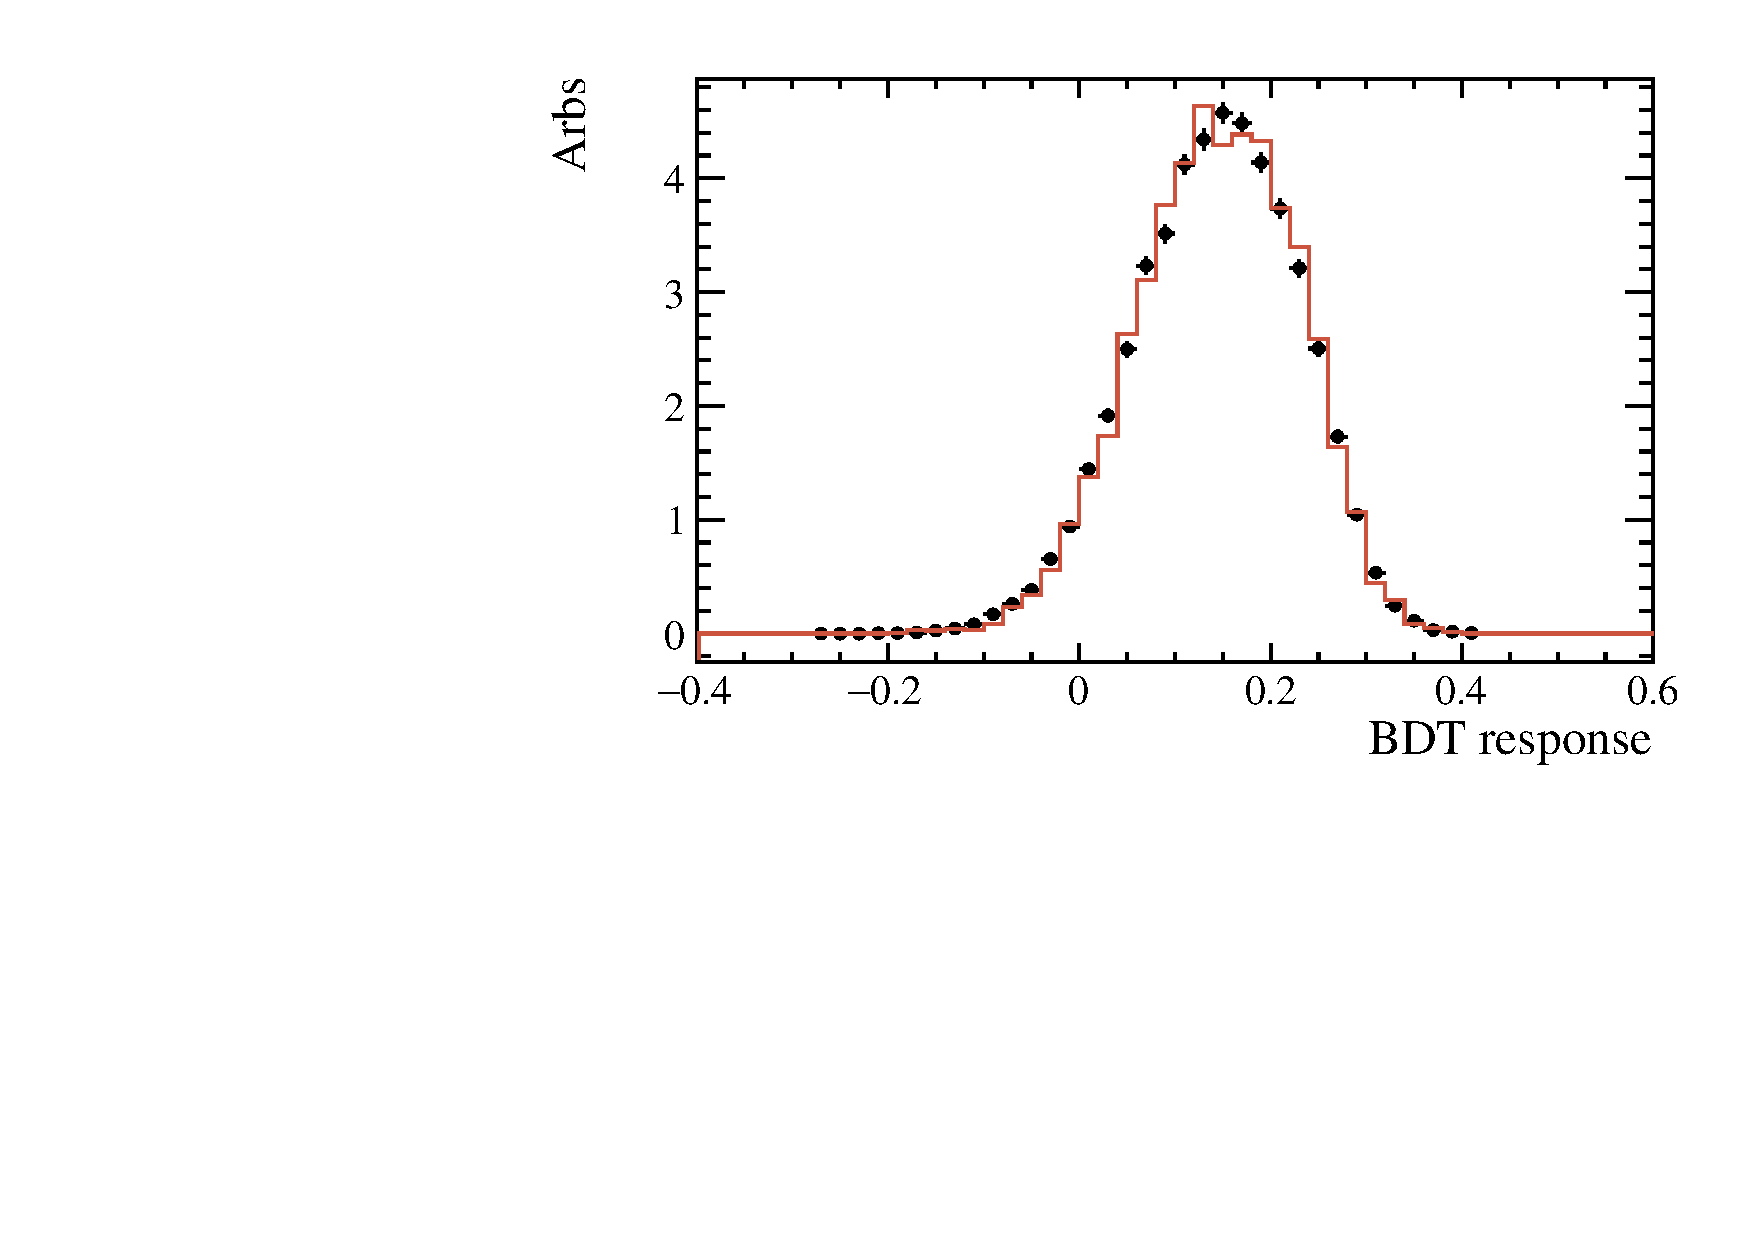
\includegraphics[width=0.48\textwidth]{bdt_k1jpsi}
    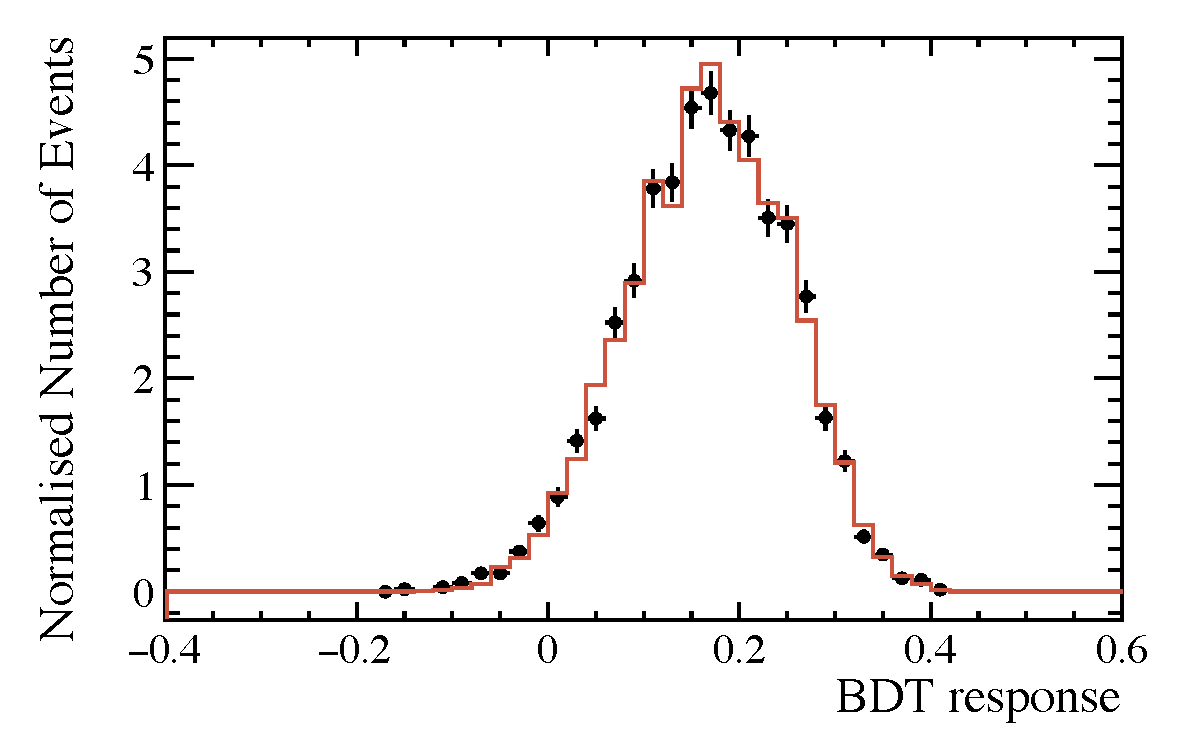
\includegraphics[width=0.48\textwidth]{bdt_psi2sk}
    \caption{\small
      Distributions of the BDT for data (black points) and simulation (red line) for the decay
      (left) \decay{\Bp}{\jpsi\kone{1270}}
      (right) \btopsitwosk.
    }
    \label{fig:kpipi:bdt}
  \end{center}
\end{figure}





